\section{Maxwell Relations \& Derivative Reduction}

\emph{Callen: Chapter 7}
\begin{itemize}
    \item Know steps for reducing derivatives
    \item Know derivative relationships and signs
    \item Given square on exam
    \item Know these are cross derivatives
\end{itemize}
There is a process to change the derivatives to a preferred set. This is mainly useful for reporting results and preferred derivatives being tabulated previously.


\textbf{The Mnemonic Diagram}
This is constructed by labeling the sides with the four common potentials ($F,G,H,U$) in alphabetical order clockwise around the diagram. The corners are labeled with the intensive parameters ($T,P$) on the right top-to-bottom and the extensive parameters ($V,S$) on the left corners top-to-bottom. Two arrows are then added to point across each diagonal to the top. The sign of the derivative is indicated by the arrow, with an arrow pointing towards the natural variable implying a positive sign. The usage of it is indicated on the next figure.

\begin{figure}[!hbtp]
    \centering
    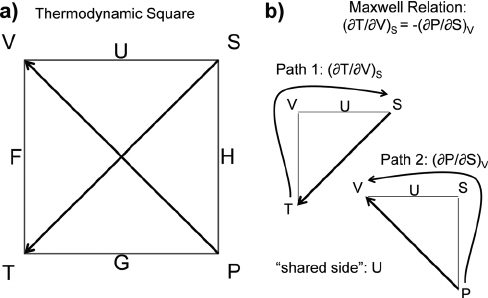
\includegraphics[scale=0.33]{Images/maxwell-square.png}
    \caption{Maxwell mnemonic square with an example.}
    \label{fig:maxwell}
\end{figure}

\newpage
\textbf{Procedure for Derivative Reduction:}

\begin{enumerate}
    \item If the derivative contains any potentials, bring them one by one to the numerator and eliminate by the thermodynamic square. ($dU=TdS-PdV+\mu dN$)
    \item If the derivative contains the chemical potential, bring it to the numerator and eliminate by means of the Gibbs-Duhem relation, $d\mu = -s dT + v dP$
    \item If the derivative contains the entropy, bring it to the numerator. If one of the four Maxwell relations of the thermodynamic square now eliminates entropy, invoke it. If not, then put a $\partial T$ under $\partial S$. The numerator will then be expressible as one of the specific heats ($c_v,c_p$).
    \item Bring the volume to the numerator. The remaining derivative will be expressible in terms of $\alpha$ and $\kappa_T$.\footnote{I have added a \hyperref[subsec::partials]{section} with information from Appendix A of Callen that describes the derivative reduction mathematically.}
    \item The originally given derivative has now been expressed in terms of the four quantities $c_v,c_p,\alpha,$ and $\kappa_T$. The specific heat at constant volume is eliminated by equation:
    \[
    c_v = c_p -Tv\alpha^2/\kappa_T
    \]
\end{enumerate}


I find this figure of an example from Wikipedia helpful.
\begin{figure}[!h]
    \centering
    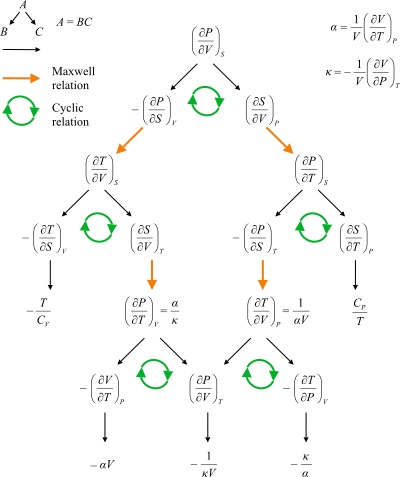
\includegraphics[scale=0.48]{Images/thermo-flow.png}
    \caption{Flow chart for thermodynamic relations.}
    \label{fig:derivflow}
\end{figure}